
\section{Definitions}

A grid edge, facet or cube is {\em active} if it contains at least one vertex 
with scalar value greater than or equal to the isovalue
and at least one vertex with scalar value less than the isovalue.

For each active grid edge $\eb$,
let $w_\eb = (1-\alpha) v_a + \alpha v_b$
where $\alpha = (\sigma - s_a)/(s_a-s_b)$
and $s_a$ and $s_b$ are the scalar values at vertices $v_a$ and $v_b$.
Point $w_\eb$ approximates the intersection of $\eb$ and the isosurface.

For each active grid cube $\cb$,
let $\cb.\centroid$ be the centroid of the points $w_\eb$
over all the active edges of $\cb$.
If the isosurface is smooth around $\cb$
and intersects $\cb$ in a single connected component,
then point $\cb.\centroid$ will lie close to the isosurface.

A grid cube with grid indices $(x_0,x_1,x_2)$ is in column $x_0$, row $x_1$
and $z$-plane $x_2$ of the grid.
Let $\cb$ and $\cb'$ be grid cubes with grid indices $(x_0,x_1,x_2)$
and $(x'_0,x'_1,x'_2)$, respectively.
The {\em cube distance} between the cubes 
is $\max(|x_0-x'_0|, |x_1-x'_1|, |x_2-x'_2|)$.
The {\em distance vector} between the cubes is
$(|x_0-x'_0|, |x_1-x'_1|, |x_2-x'_2|)$.

For a grid cube $\cb$, region $\RIII_\cb$ is the $3 \times 3 \times 3$ region
of 27 grid cubes centered at $\cb$.
Region $\RV_\cb$ is the $5 \times 5 \times 5$ region
of 125 grid cubes centered at $\cb$.


\begin{figure}
\begin{equation*}
\xymatrix{
\action{Compute isosurface vertex locations} \ar[d] \\
\action{Select well-spaced subset of vertices on sharp features} \ar[d] \\
\action{Merge isosurface vertices around selected vertices}
}
\end{equation*}
\caption{Algorithm SHREC.}
\label{alg:shrec}
\end{figure}


\begin{algorithm}[t]
\tcc{$C_d$ = cubes generating vertices on $d$-dimensional features}
Sort $C_0$ and $C_1$ by increasing $|\cb.\isov-\cb.\centroid|$\;
Mark all cubes as uncovered\;
\ForEach{cube $\cb$ of $C_0$}{
\label{step:A}
\If{(cube $\cb$ is uncovered)}{
\If{($\cb.\isov$ does not create a large
angle triangle with vertices from previously selected cubes)}{
\label{step:largeAngle}
Select $\cb$\;
\ForEach{cube $\cb'$ sharing a vertex with $\cb$}{
Mark $\cb'$ as covered\;
}
}
}
}
\label{step:B}
Repeat steps~\ref{step:A}-\ref{step:B} on $C_1$\;
\caption{Selection of feature cubes in MergeSharp.}
\label{alg:mergesharp_select}
\end{algorithm}


\begin{figure}[t]
\centering

\begin{tabular}{cc}
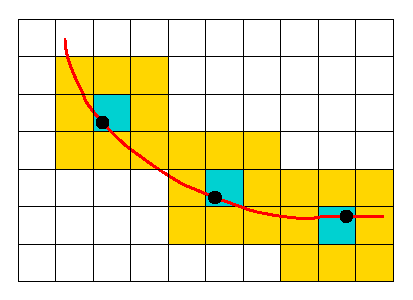
\includegraphics[width=0.4\linewidth]{images/selectA.eps} \qquad &
\qquad
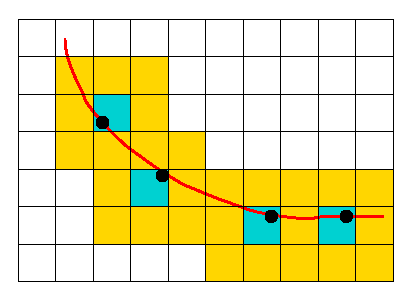
\includegraphics[width=0.4\linewidth]{images/selectB.eps} \\
(a) & (b) 
\end{tabular}

\caption{2D illustration of vertex and cube selection.
(a) Selection which gives poor cover of the red curve.
The curve intersects an uncovered square.
(b) Selection which gives better cover of the red curve.
The curve is far away from any uncovered square.
}
\label{fig:select}
\end{figure}


\section{MergeSharp}
\label{section:mergesharp}

Algorithm SHREC has three parts:
computation of isosurface vertex locations, 
selection of a well-spaced subset of vertices on sharp features
and merging of vertices around selected vertices
(Figure~\ref{alg:shrec}).
Algorithm MergeSharp from~\cite{bw-cisec-13} 
has a similar three parts,
but each part is substantially different in SHREC.
To motivate the description of Algorithm SHREC,
we briefly describe each part in MergeSharp and the associated problems.

In the first part, 
MergeSharp computes the location of an isosurface vertex, $\cb.\isov$,
in or near each active grid cube $\cb$.
MergeSharp computes this location using gradients at the vertices of $\cb$
and cubes adjacent to $\cb$.
When cube $\cb$ is near a sharp feature,
the isosurface vertex will lie on that feature.
MergeSharp also identifies whether the feature 
is 0-dimensional or 1-dimensional
or if the vertex lies on a smooth region of the isosurface.

In the second part, MergeSharp selects a subset of the isosurface vertices
lying on 0 or 1-dimensional features.
These vertices will form the sharp feature in the isosurface mesh.
Cubes which generate such vertices are called {\em selected} cubes.
MergeSharp chooses selected cubes as follows.

Let $C_0$ and $C_1$ be the set of cubes whose isosurface vertices
lie on 0-dimensional features or 1-dimensional features, respectively.
Mark all the cubes as ``uncovered''.
Sort $C_0$ and $C_1$ by increasing distance
of $\cb.\isov$ from $\cb.\centroid$.
Select the next uncovered cube $\cb$ in $C_0$
where $p_\cb$ does not form a large angle triangle 
with vertices in previously selected cubes.
Mark all cubes which share a vertex with $\cb$ as covered.
After processing list $C_0$, apply the same procedure to list $C_1$.
Pseudocode is given in Figure~\ref{alg:mergesharp_select}.

The third part is merging covered cubes with selected cubes.
MergeSharp simply merges each covered cube with the first selected cube
which covers it.
In the description of MergeSharp in~\cite{bw-cisec-13}, 
the selection and merging steps are combined
so that a cube is merged as soon as it is covered,
but the outcome of the algorithm is exactly the same.

There are problems with every one of the three steps of MergeSharp.
First, MergeSharp uses gradients from $\cb$ or its immediate neighbors
to compute the location of $\cb.\isov$.
As discussed in~\cite{bw-isifsd-15},
computing correct gradients near sharp features is difficult,
if not impossible.
Thus, the gradients in $\cb$ and its neighbors may not be known.
Algorithm SHREC selects gradients from a larger area
than just the immediate neighbors of $\cb$.

Second, the isosurface vertex $\cb.\isov$ generated by cube $\cb$
may lie outside $\cb$.
Moreover, if cube $\cb$ is near a 1-dimensional feature,
point $\cb.\isov$ may lie outside of $\cb$
even if this 1-dimensional feature intersects $\cb$.
In addition, because of curvature, noise and numerical instability,
point $\cb.\isov$ could lie in some cube $\cb'$ adjacent to $\cb$
while point $\cb'.\isov$ lies inside $\cb.\isov$.
Algorithm SHREC locates $\cb.\isov$ inside $\cb$ whenever possible.

Third, the selection step chooses cubes based on the proximity
of $\cb.\isov$ to $\cb.\centroid$.
If a point $\cb.\isov$ is near $\cb.\centroid$,
it probably is located in cube $\cb$ 
and is a good approximation of the vertex location.
While this is reasonable,
it ignores the interaction between selected cubes.
MergeSharp does better when 1-dimensional features are well-covered 
by the selected and covered cubes.
For instance, in the 2D illustration in Figure~\ref{fig:select}, 
the selected squares are packed together more closely
and their $3 \times 3$ regions do a better job of covering
the given curve.
Algorithm SHREC selects cubes so that they are packed closely together.

Finally, the merging step merges cube $\cb$
with the the first selected cube adjacent to $\cb$.
Doing so sometimes distorts triangles, creating extremely thin triangles
and sometimes creating ``folds'' in the surface mesh.
Algorithm SHREC prefers merging cubes which are facet
adjacent over merging edge adjacent or vertex adjacent cubes.
It also avoids merges which creates small thin triangles or creates folds.
It extends the merging by one more cube in certain regions
to ensure good covering of 1D features.


\begin{figure}
\begin{equation*}
\xymatrix{
\action{Compute $\cb.\isovLoc$ for each active cube $\cb$.} \ar[d] \\
\action{If $\cb.\isovLoc$ is in $\cb'$ while $\cb'.\isovLoc$ is in $\cb$,\\
swap $\cb.\isovLoc$ and $\cb'\isovLoc$.} \ar[d] \\
\action{If $\cb.\isovLoc$ is in $\cb'$,
then $\cb'\isovLoc \leftarrow \cb.\isovLoc$.} \ar[d] \\
\action{If $\cb$ and $\cb'$ are 1D feature cubes intersecting 
in a grid edge $\eb$,\\
then compute the intersection $p$ of $\cb.\Lsharp$ 
and a plane separating $\cb$ and $\cb'$.\\
$\tcb.\isov \leftarrow p$ where $\tcb$ is the cube containing $p$.} 
\ar[d] \\
\action{If $\cb$ and $\cb'$ are 1D feature cubes intersecting 
in a grid vertex $v$,\\
then compute the intersection $p$ of $\cb.\Lsharp$ 
and a plane separating $\cb$ and $\cb'$.\\
$\tcb.\isov \leftarrow p$ where $\tcb$ is the cube containing $p$.} 
}
\end{equation*}
\caption{SHREC algorithm for generating points on sharp features.}
\label{alg:shrec_isov}
\end{figure}

\section{Generating Points on Sharp Features}
\label{section:generation}

As noted in Section~\ref{section:mergesharp},
when a cube $\cb$ intersects a 1-dimensional feature,
we would like to choose a point $\cb.\isov$ inside that feature 
whenever possible.
We would also like that point to be ``near'' the center
of the intersection of the isosurface and cube $\cb$.
Finally, if the 1-dimensional feature is near $\cb$ 
but does not intersect $\cb$,
we would like to choose a point that is ``closest'' to $\cb$.

SHREC uses a number of techniques to compute points inside cubes.
First, when a cube $\cb$ is near a 1-dimensional feature,
SHREC computes a line $\cb.\Lsharp$ approximating the feature near $\cb$.
SHREC computes the points on $\cb.\Lsharp$ closest to $\cb.\centroid$
and $\cb.\centerVar$.
If one of those points is inside $\cb$,
then SHREC sets $\cb.\isov$ to that point.
Otherwise, SHREC computes the point on $\cb.\Lsharp$ 
which is closest to $\cb.\centerVar$ under the $L_\infty$ metric.
If $\cb.\Lsharp$ intersects $\cb$, then that point will lie in $\cb$.

Second, SHREC compares isosurface vertex locations 
computed by neighboring cubes and swaps or sets isosurface vertex locations
based on those comparisons.
Third, SHREC computes isosurface vertex locations on planes
separating cubes intersecting 1D features.
SHREC stores these isosurface vertex locations in the cubes containing them.

The second and third steps of the algorithm are outlined 
in Figure~\ref{alg:shrec_isov}.
Details of all three steps follow.


\subsection{Computing Isosurface Vertex Locations}
\label{section:loc}

At the heart of any algorithm to compute a surface with sharp features 
is an algorithm to compute the locations of mesh vertices on those features.
SHREC uses the algorithm from MergeSharp~\cite{bw-cisec-13}
to compute an initial vertex location $\cb.\isovLoc$ 
for each active cube $\cb$.
The algorithm computes the vertex locations 
from gradients at grid vertices.
The MergeSharp algorithm is a variation 
of the algorithms in~\cite{jlsw-dchd-02,kbsh-fssev-01,sw-dcss-02,zhk-dctps-04}
for computing vertex locations from surface normals.

SHREC computes one isosurface vertex location $\cb.\isovLoc$
for each active grid cube $\cb$.
The algorithm computes an isosurface vertex location for $\cb$
by using the gradients at vertices of $\cb$ and nearby cubes.
A grid vertex $v$ with scalar $s_{v}$ and gradient $g_{v}$ gives a plane
\begin{equation}
\label{eqn:isoplane}
h_v = \{p : (p-v) \cdot g_{v} + s_{v}= \sigma \}.
\end{equation}
This plane is an ``approximation'' to the tangent planes to the isosurface
at isosurface points in the neighborhood of $v$.

A set of $k$ vertices and gradients gives a set of $k$ equations 
in three variables $M p = b$
where $M$ is a $k \times 3$ matrix 
and $b$ is a column vector with $k$ rows 
and the unknown $p$ is a column vector with three rows.
Of course, if $M$ has more than three rows,
the system $Mp = b$ is over-determined and has no exact solution.
The least squares approximation to $M p = b$ 
is the solution to $M^T M p = M^T b$.

Let $A$ be the $3 \times 3$ matrix $M^T M$ and 
let $b'$ equal the column vector $M^T b$.
SHREC uses singular valued decomposition (SVD)
as described in~\cite{jlsw-dchd-02,kbsh-fssev-01,l-oslpm-00}
to compute an isosurface vertex location from the equation $A p = b'$.

Let $\sigma_1$, $\sigma_2$ and $\sigma_3$ be the singular values of $A$
sorted in decreasing order.
A singular value $\sigma_i$ is {\em large},
if $\sigma_i/\sigma_1 \ge \epsilon$ for some predefined parameter $\epsilon$.
There are three possible cases based on the number of large singular values
of $A$.
In the first case $A$ has three large singular values.
In this case, the tangent planes around $\cb$ have normals in three or more
very distinct directions.
The isosurface has some 0-dimensional feature near cube $\cb$.
We call a cube $\cb$ a {\em 0D feature cube} if the matrix $A$ associated
with $\cb$ has three large singular values.
The solution to $A p = b'$ approximates the 0-dimensional feature 
near cube $\cb$.

In the second case, matrix $A$ has only two large singular values.
In this case, 
the tangent plane normals are close to two different directions.
The isosurface has some 1-dimensional feature near cube $\cb$.
We call a cube $\cb$ a {\em 1D feature cube} if the matrix $A$ associated
with $\cb$ has two large singular values.

To compute the 1-dimensional feature near $\cb$,
we use singular valued decomposition to remove the small singular value
from $A$.
The singular valued decomposition of $A$ is $A = U \Sigma V^T$
where
\begin{equation*}
\Sigma = \left (
\begin{array}{ccc}
\sigma_1 & 0 & 0 \\
0 & \sigma_2 & 0 \\
0 & 0 & \sigma_3
\end{array}
\right )
.
\end{equation*}
When $A$ has only two large singular values, $\sigma_1$ and $\sigma_2$,
MergeSharp replaces $\Sigma$ by a new diagonal matrix $\Sigma'$
with diagonal entries $\sigma_1$, $\sigma_2$, 0.
Let $A'$ equal $U \Sigma' V^T$.
Matrix $A'$ has rank two.
The solution to $A' p = b'$ is a set of points on a line $\cb.\Lsharp$.
Line $\cb.\Lsharp$ represents a line tangent to the 1-dimensional feature.

In the last case,
matrix $A$ has only one large singular value.
In this case, the tangent plane normals are close to a single direction.
The isosurface is smooth around cube $\cb$.
Replace $\Sigma$ by a new diagonal matrix $\Sigma'$
with diagonal entries $\sigma_1$, 0, 0.
Let $A'$ equal $U \Sigma' V^T$.
Matrix $A'$ has rank one.
The solution to $A' p = b'$ is a set of points on a plane.
That plane represents a tangent plane to the isosurface in cube $\cb$.

In the case that $A$ has only one or two large singular values,
the solution to $A' p = b'$ is a line or plane.
As suggested in~\cite{sw-dcss-02},
SHREC selects the point on the line or plane that is closest 
to $\cb.\centroid$.

More precisely, SHREC defines the diagonal matrix $\Sigma^+$
with diagonal entries:
\begin{equation*}
\begin{array}{ll}
1/\sigma_1, 1/\sigma_2, 1/\sigma_3, 
  & \mbox{ if $A$ has three singular values,}\\
1/\sigma_1, 1/\sigma_2, 0, 
  & \mbox{ if $A$ has two singular values,}\\
1/\sigma_1, 0, 0, 
  & \mbox{ if $A$ has one singular value.}
\end{array}
\end{equation*}
The point
\begin{equation}
\label{eqn:Lindstrom}
\phi_\cb(q) = q + V \Sigma^+ U^T (b' - A \, q) 
\end{equation}
is the point on $\{p: A' p = b'\}$ closest to $q$.
SHREC selects point $\phi_\cb(\cb.\centroid)$
on the line or plane $\{p: A'p = b'\}$.

The number of large singular values of $A$ determines
whether the computed isosurface vertex location lies 
on a 0-dimensional feature, a 1-dimensional feature, 
or a smooth portion of the isosurface.
This information is used in subsequent steps in the SHREC algorithm.

When $A' p = b'$ is a line,
the direction of that line is given by the equation $(I - V \Sigma^+ U^T ) w$
for any vector $w$ which is not in the kernel of $(I - V \Sigma^+ U^T ) w$.
Substituting $(1,0,0)$, $(0,1,0)$ and $(0,0,1)$ for $w$
and using $(I - V \Sigma^+ U^T ) w$ with largest magnitude
gives the direction.
The direction and point $\phi_\cb(\centroid)$ defines the line $\cb.\Lsharp$.

Instead of using $A = M^T M$,
we could have used the singular value decomposition of $M$.
Using $M$ is preferable for numerical stability,
since the condition number of $A$ is the square of the condition number of $M$.
However, because we remove small eigenvalues,
the numerical stability is not an issue.
We use the singular value decomposition of the $3 \times 3$ matrix $A$
because it is simpler and faster to compute 
than the singular valued decomposition of the $k \times 3$ matrix $M$.


\begin{figure}[t]
\centering

\begin{tabular}{cc}
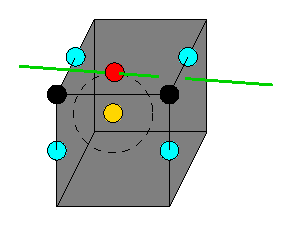
\includegraphics[width=0.4\linewidth]{images/centroid.eps} \qquad &
\qquad
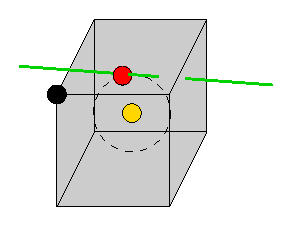
\includegraphics[width=0.4\linewidth]{images/center.eps} \\
(a) & (b)
\end{tabular}

\caption{Green line is $\cb.\protect\Lsharp$.
Black cube vertex has scalar value above the isovalue.
(a) Red point is point on $\cb.\protect\Lsharp$ closest 
to $\cb.\protect\centroid$ (yellow).
Green line $\cb.\protect\Lsharp$ intersects cube $\cb$
but red point is outside cube $\cb$.
Blue points are the intersection points of the isosurface
and the cube edges, computed using linear interpolation.
(b) Red point is point on $\cb.\protect\Lsharp$ closest 
to $\cb.\protect\centerVar$ (yellow).
Green line $\cb.\protect\Lsharp$ intersects cube $\cb$
but red point is outside cube $\cb$.
}
\label{fig:out_of_cube}
\end{figure}

\subsection{Computing Vertex Locations on 1-Dimensional Features}

Consider a 1D feature cube $\cb$.
By definition, cube $\cb$ is near some 1-dimensional feature.
That 1D feature is approximated by the line $\cb.\Lsharp$.
The location $\cb.\isovLoc$ of the isosurface vertex associated with $\cb$ 
should be on $\cb.\Lsharp$.
However, that condition still gives one degree of freedom in selecting
the location of $\cb.\isovLoc$.
One obvious additional condition is that if $\cb.\Lsharp$ intersects $\cb$,
then $\cb.\isovLoc$ should be in $\cb$.
An additional condition is that if $\cb.\Lsharp$ does not intersect $\cb$,
then $\cb.\isovLoc$ should be ``close to'' $\cb$ 
under some suitably defined metric.

Algorithm SHREC computes three different possible isosurface vertex locations.
First, Algorithm SHREC computes the point $p^0_\cb = \phi_\cb(\cb.\centroid)$
(Equation~\ref{eqn:Lindstrom}),
the point on $\cb.\Lsharp$ which is closest to $\cb.\centroid$.
The idea is that $\cb.\centroid$ is a good approximation
for the intersection of $\cb$ and the isosurface,
and so one should choose a point near $\cb.\centroid$.
If $p^0_\cb$ lies in $\cb$, then SHREC sets $\cb.\isovLoc$ to $p^0_\cb$.

In most cases, if line $\cb.\Lsharp$ intersects cube $\cb$.
then the point $p^0_\cb$ will lie in $\cb$.
However, if line $\cb.\Lsharp$ is ``near'' some facet or edge of $\cb$,
then it is possible for $\cb.\Lsharp$ to intersect $\cb$
but $p^0_\cb$ to lie outside $\cb$.
(See Figure~\ref{fig:out_of_cube}(a).)

If $p^0_\cb$ lies outside $\cb$,
then SHREC computes $p^1_\cb = \phi_\cb(\cb.\centerVar)$, 
the point on $\cb.\Lsharp$ which lies closest 
to the center $\cb.\centerVar$ of cube $\cb$.
If $p^1_\cb$ is in $\cb$ while $p^0_\cb$ is not,
SHREC sets $\cb.\isovLoc$ to $p^1_\cb$.

Unfortunately, it is possible that both $p^0_\cb$ and $p^1_\cb$
are not in $\cb$ even though $\cb.\Lsharp$ intersects $\cb$.
(See Figure~\ref{fig:out_of_cube}(b).)
As a final step, SHREC computes a point $p^2_\cb$ on $\cb.\Lsharp$ 
which is closest to the center $\cb.\centerVar$ of $\cb$ 
under the $L_\infty$ metric.
If $\cb.\Lsharp$ intersects $\cb$, 
then this point is guaranteed to lie in $\cb$.
Details for computing $p^2_\cb$ are in Appendix~\ref{appendix:Linf}.
If $p^2_\cb$ is in $\cb$ while $p^1_\cb$ and $p^2_\cb$ are not,
SHREC sets $\cb.\isovLoc$ to $p^2_\cb$.

Instead of computing $p^0_\cb$, $p^1_\cb$ and $p^2_\cb$,
we could compute and use only $p^2_\cb$.
However, the computations of $p^0_\cb$ and $p^1_\cb$ and $p^2_\cb$ 
are much faster,
and their locations are preferable to $p^2_\cb$ when they are
contained in cube $\cb$.
Algorithm MergeSharp computes only $\phi^0_\cb$.


\begin{figure}[t]
\centering

\begin{tabular}{cc}
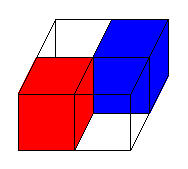
\includegraphics[width=0.4\linewidth]{images/shared_edge.eps} \qquad &
\qquad
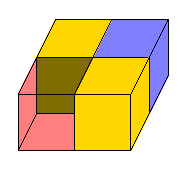
\includegraphics[width=0.4\linewidth]{images/shared_edge_B.eps} \\
(a) & (b)
\end{tabular}

\caption{(a) Two grids cubes sharing an edge $\eb$.
(b) The two other cubes (yellow) which also contain $\eb$.
}
\label{fig:shared_edge}
\end{figure}

\begin{figure}[t]
\centering

\begin{tabular}{cc}
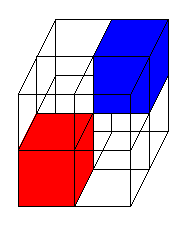
\includegraphics[width=0.4\linewidth]{images/shared_vertex.eps} \qquad &
\qquad
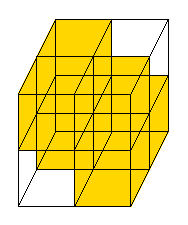
\includegraphics[width=0.4\linewidth]{images/shared_vertex_B.eps} \\
(a) & (b)
\end{tabular}

\caption{(a) Two grids cubes sharing a vertex $v$.
(b) The six other cubes (yellow) which also contain $v$.
}
\label{fig:shared_vertex}
\end{figure}

\subsection{Swapping Locations}

Many of the problems in Algorithm SHREC (and MergeSharp) occur when
isosurface vertex location $\cb.\isovLoc$ lies outside of cube $\cb$.
Thus, it is always preferable that $\cb.\isovLoc$ be in $\cb$.
This is not always possible since the sharp features near $\cb$
may not intersect $\cb$.
However, in cases where a sharp feature intersects $\cb$,
we would like $\cb.\isovLoc$ to be in $\cb$.

The computation of a sharp feature near $\cb$ depends
upon gradients in the neighborhood of $\cb$.
The set of such gradients changes for each cube $\cb$.
Because of the inaccuracy in computing sharp features,
it is possible that $\cb.\isovLoc$ is in a cube $\cb'$ adjacent to $\cb$
while $\cb'.\isovLoc$ is not contained in $\cb$.
In some cases,
location $\cb.\isovLoc$ is in $\cb'$ while $\cb'.\isovLoc$ is in $\cb$.
In those cases,
we simply swap $\cb.\isovLoc$ and $\cb'.\isovLoc$.
In other cases, location $\cb'.\isovLoc$ lies in some third cube $\cb''$.
In that case, we simply set $\cb'.\isovLoc$ to $\cb.\isovLoc$.

The setting of isosurface vertex locations from adjacent cubes
increases the number of cubes $\cb$ containing 
their associated vertext locations $\cb.\isovLoc$.
Note that if the initial location $\cb.\isovLoc$ lies in $\cb$,
then we never change $\cb.\isovLoc$.


\subsection{Locations on Planes}

Consider two grid cubes, $\cb$ and $\cb'$, 
which intersect in an edge $\eb$ but not in any facet.
(See Figure~\ref{fig:shared_edge}.)
Two other grid cubes, $\tcb$ and $\tcb'$ share edge $\eb$.
A 1-dimensional feature which passes through $\cb$ and $\cb'$ must intersect
either $\tcb$ or $\tcb'$.
(In the exceptional case, the 1-dimensional featuer passes through $\eb$,
in which case it intersects both $\tcb$ and $\tcb'$.)
Since the 1D feature intersects either $\tcb$ and $\tcb'$,
either $\tcb.\isovLoc$ should be in $\tcb$ 
or $\tcb'.\isovLoc$ should be in $\tcb'$.
However, because of inaccuracies in computing points on 1D features,
neither condition may hold.

To ensure that either $\tcb.\isovLoc$ lies in $\tcb$
or $\tcb'.\isovLoc$ lies in $\tcb'$,
Algorithm SHREC computes the plane $h$ containing $\eb$
and perpendicular to the line from $\cb.\centerVar$ to $\cb'.\centerVar$.
SHREC then computes the intersection of the line $\cb.\Lsharp$ 
and plane $h$.
This intersections point, $p_I$, lies in either $\tcb$ or $\tcb'$.
If $p_I$ lies in $\tcb$ and $\tcb.\isovLoc$ is not in $\tcb$,
SHREC sets $\tcb.\isovLoc$ to $p_I$.
If $p_I$ lies in $\tcb'$ and $\tcb'.\isovLoc$ is not in $\tcb'$,
SHREC sets $\tcb'.\isovLoc$ to $p_I$.

Next, consider the case of two grid cubes, $\cb$ and $\cb'$, 
which intersect in a vertex $v$ but not in any edge.
(See Figure~\ref{fig:shared_vertex}.)
Six other grid cubes share vertex $v$ with $\cb$ and $\cb'$.
A 1-dimensional feature which passes through $\cb$ and $\cb'$ must intersect
one of these six other grid cubes.
(In the exceptional case, the 1D feature passes through $v$,
in which case all six.)
Since the 1D feature intersects one of the six grid cubes,
point $\tcb.\isovLoc$ should lie in $\tcb$ for one of the six grid cubes $\tcb$.
Again because of inaccuracies in computing points on 1D features,
point $\tcb.\isovLoc$ may not be in $\tcb$ for any of the six grid cubes $\tcb$.

To ensure that $p_\tcb$ lies in $\tcb$ for one of the six grid cubes,
Algorithm SHREC computes the plane $h$ containing $v$
and perpendicular to the line from $\cb.\centerVar$ to $\cb'.\centerVar$.
SHREC then computes the intersection of the line $\cb.\Lsharp$ and plane $h$.
This intersections point, $p_I$, lies in at least one of the six grid cubes.
If $p_I$ lies in cube $\tcb$ and $\tcb.\isovLoc$ is not in $\tcb$,
SHREC sets $\tcb.\isovLoc$ to $p_I$.

The computation in this section ensures ``continuity'' in the cubes
which intersect a 1-dimensional feature
If a 1-dimensional feature intersects a cube $\cb$,
then the 1-dimensional feature should intersect two cubes $\cb'$ and $\cb''$
which share a facet with $\cb$.
SHREC's computation of line-plane intersections described above,
ensures that if $\cb'$ and $\cb''$ are active cubes,
then $\cb'$ will contain $\cb'.\isovLoc$ and 
$\cb''$ will contain $\cb''.\isovLoc$.


\begin{figure}
\centering
\begin{tabular}{cc}
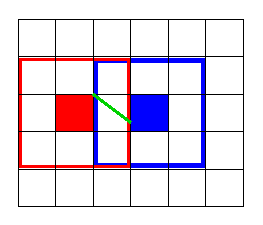
\includegraphics[width=1.2in]{images/config2D_2_0.eps} \qquad &
\qquad
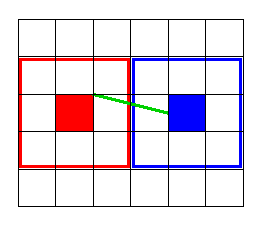
\includegraphics[width=1.2in]{images/config2D_3_0.eps} \\
(a) Configuration (2,0). & (b) Configuration (3,0). \\
\\
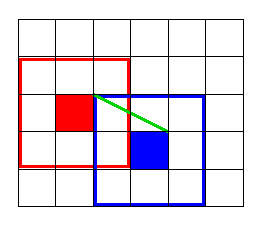
\includegraphics[width=1.2in]{images/config2D_2_1.eps}
\qquad &
\qquad
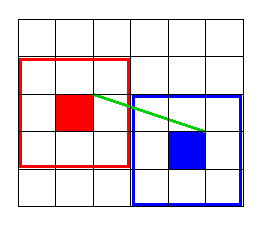
\includegraphics[width=1.2in]{images/config2D_3_1.eps} \\
(c) Configuration (2,1). & (d) Configuration (3,1).
\end{tabular}
\caption{Tightly packed 2D configurations of selected squares.
Selected squares and $3 \times 3$ region around each square.
Line segments with endpoints on the two selected squares 
(e.g., the green line segments) are contained
within the union of the two $3 \times 3$ regions.}
\label{fig:packed2D}
\end{figure}

\begin{figure}[t]
\centering
\begin{tabular}{cc}
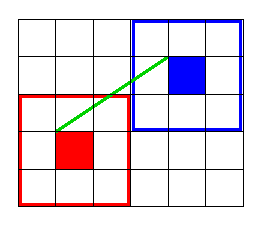
\includegraphics[width=1.2in]{images/config2D_3_2.eps} \qquad &
\qquad
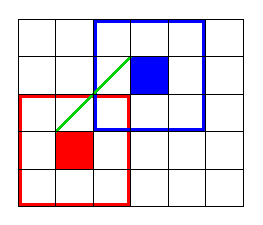
\includegraphics[width=1.2in]{images/config2D_2_2.eps} \\
(a) Configuration (3,2). & (b) Configuration (2,2).
\end{tabular}
\caption{Problematic 2D configurations of selected squares.
Selected squares and $3 \times 3$ region around each square.
(a) The green line segment is not contained within the union
of the two $3 \times 3$ regions.
(b)~The green line segment intersects the boundary
of the union of the two $3 \times 3$ regions.}
\label{fig:loose2D}
\end{figure}

\begin{figure}[t]
\centering
\begin{tabular}{cc}
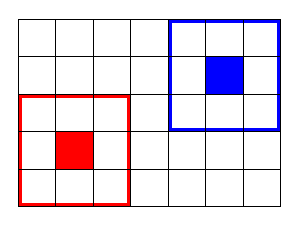
\includegraphics[width=1.2in]{images/config2D_4_2.eps} \qquad &
\qquad
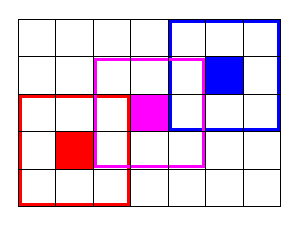
\includegraphics[width=1.2in]{images/config2D_4_2_B.eps} \\
(a) Configuration (4,2). & (b) Additional cube.
\end{tabular}
\caption{(a) Configuration (4,2) has space between the $3 \times 3$
regions around each selected square.
(b) Additional cube (magenta) which packs tightly with two other squares.}
\label{fig:config2D_4_2}
\end{figure}

\begin{figure*}
\centering
\begin{tabular}{cccc}
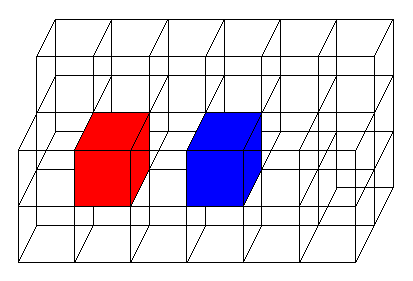
\includegraphics[width=1.2in]{images/config3D_2_0_0.eps} \qquad &
\qquad
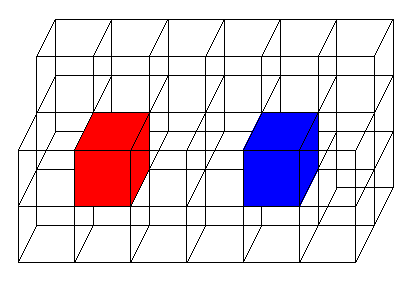
\includegraphics[width=1.2in]{images/config3D_3_0_0.eps}
\qquad &
\qquad
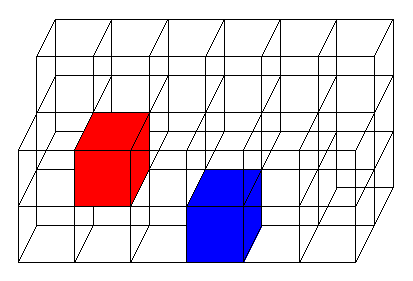
\includegraphics[width=1.2in]{images/config3D_2_1_0.eps}
\qquad &
\qquad
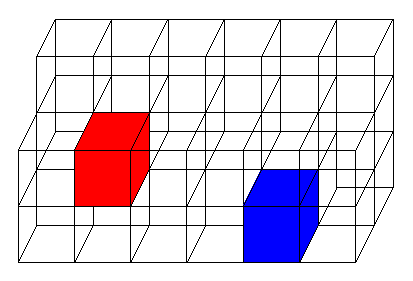
\includegraphics[width=1.2in]{images/config3D_3_1_0.eps} \\
(a) Configuration (2,0,0). & (b) Configuration (3,0,0). 
  & (c) Configuration (2,1,0). & (d) Configuration (3,1,0).\\
\\
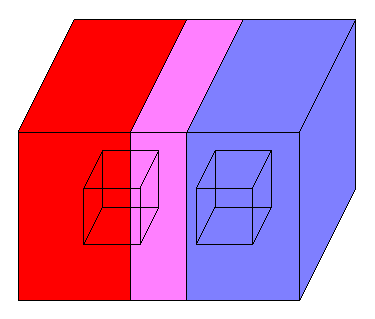
\includegraphics[width=1.2in]{images/config3D_2_0_0_3x3x3.eps} \qquad &
\qquad
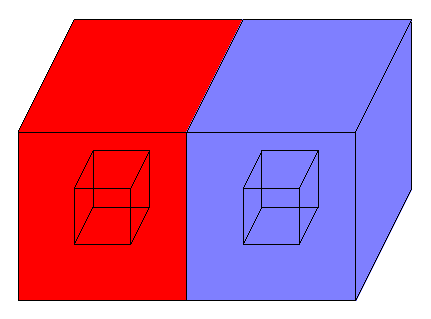
\includegraphics[width=1.2in]{images/config3D_3_0_0_3x3x3.eps}
\qquad &
\qquad
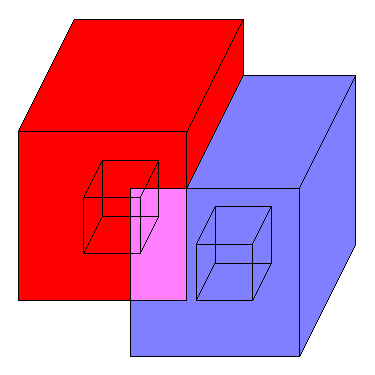
\includegraphics[width=1.2in]{images/config3D_2_1_0_3x3x3.eps}
\qquad &
\qquad
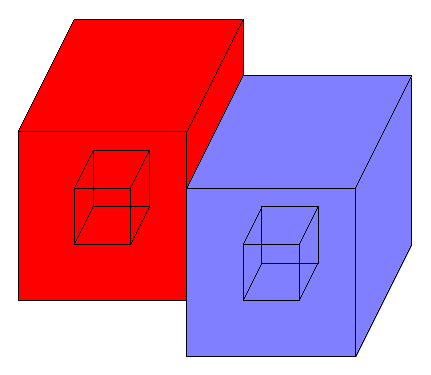
\includegraphics[width=1.2in]{images/config3D_3_1_0_3x3x3.eps} \\
(e) $\gDim{3}$ regions. & (f) $\gDim{3}$ regions. 
  & (g) $\gDim{3}$ regions. & (h) $\gDim{3}$ regions.\\
Configuration (2,0,0). & Configuration (3,0,0). 
  & Configuration (2,1,0). & Configuration (3,1,0).
\end{tabular}
\caption{Tightly packed 3D configurations of selected cubes.}
\label{fig:packed3D}
\end{figure*}


\section{Selecting 0D and 1D Feature Cubes}
\label{section:selection}

Algorithm SHREC selects a well-spaced subset 
of the 0D and 1D feature cubes
and merges isosurface vertices in adjacent cubes 
with the vertices generated by the selected cubes.
To ensure that the isosurface vertices on sharp features are well-spaced,
SHREC never selects two cubes which have a common vertex.
Whenever SHREC selects a cube $\cb$,
any adjacent cube sharing a vertex with $\cb$ is marked as ``covered''
by $\cb$.
SHREC never selects a covered cube.

SHREC follows a MergeSharp rule in never selecting a cube $\cb$
if $\cb.\isov$ creates a large angle triangle 
(Algorithm~\ref{alg:mergesharp_select}, step~\ref{step:largeAngle})
with vertices from previously selected cubes.
SHREC does not select cube $\cb$
if $\cb.\isov$ creates such a triangle with angle $140^\circ$ or greater.

As noted in Section~\ref{section:mergesharp}, 
SHREC does better when selected cubes 
are packed ``tightly'' together.
(See also Figure~\ref{fig:select}.)
In particular, SHREC tries to avoid certain configurations of nearby cubes.

Consider cubes $\cb$ and $\cb'$ with grid indices $(x_0,x_1,x_2)$
and $(x'_0,x'_1,x'_2)$, respectively.
(A cube with grid indices $(x_0,x_1,x_2)$ is in column $x_0$, row $x_1$
and $z$-plane $x_2$ of the grid.)
The {\em distance vector} between the cubes is
$(|x_0-x'_0|, |x_1-x'_1|, |x_2-x'_2|)$.
Two grid cubes are in configuration $(a_0,a_1,a_2)$ if the distance vector
between the cubes is some permutation of $(a_0,a_1,a_2)$.
Figures~\ref{fig:packed2D}, \ref{fig:loose2D}, \ref{fig:config2D_4_2}
and~\ref{fig:packed3D},
contain examples of 2D and 3D configurations of grid cubes.

We can get some insight into 3D configurations of grid cubes
by considering the 2D configurations of grid squares.
Figure~\ref{fig:packed2D} contains configurations $(2,0)$, $(3,0)$,
$(2,1)$ and $(3,1)$ of grid squares.
The $3 \times 3$ regions around the selected squares are ``tightly packed''
so that any line segment with endpoints in the selected squares
is contained within the union of the two $3 \times 3$ regions.

Figure~\ref{fig:loose2D} contains configurations $(3,2)$ and $(2,2)$
of grid squares.
With configuration $(3,2)$, some line segments with endpoints
in the selected squares are not contained within the union
of the $3 \times 3$ regions.
Configuration $(2,2)$ is somewhat better,
since all line segments with endpoints in the selected squares
are contained within the union of the $3 \times 3$ regions.
Unfortunately, they are only barely contained.
The green line segment in Figure~\ref{fig:loose2D}(b) intersects
the boundary of the $3 \times 3$ region.
Slightly curving the segment could mean that it no longer was contained
in the union.

Note that if selected squares are suitably far apart,
then additional squares can be selected between them.
For instance, a magenta square can be selected between the two colored squares
in Figure~\ref{fig:config2D_4_2}(a) and the $3 \times 3$ regions
will fit together tightly.

\begin{figure*}
\centering

\begin{tabular}{ccc}
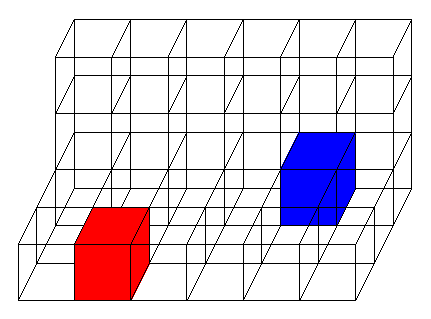
\includegraphics[width=1.2in]{images/config3D_3_2_0.eps} \qquad &
\qquad
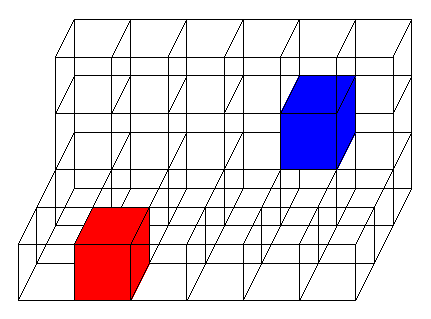
\includegraphics[width=1.2in]{images/config3D_3_2_1.eps}
\qquad &
\qquad
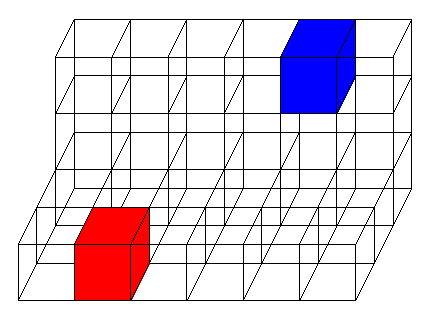
\includegraphics[width=1.2in]{images/config3D_3_2_2.eps} \\
(a) Configuration (3,2,0). & (b) Configuration (3,2,1). 
  & (c) Configuration (3,2,2).\\
\\
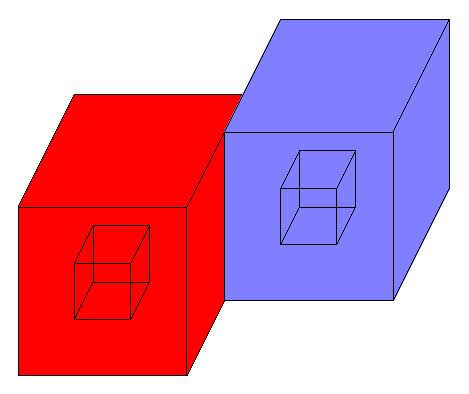
\includegraphics[width=1.2in]{images/config3D_3_2_0_3x3x3.eps} \qquad &
\qquad
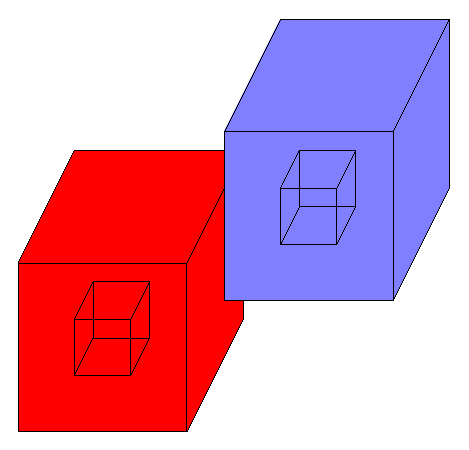
\includegraphics[width=1.2in]{images/config3D_3_2_1_3x3x3.eps}
\qquad &
\qquad
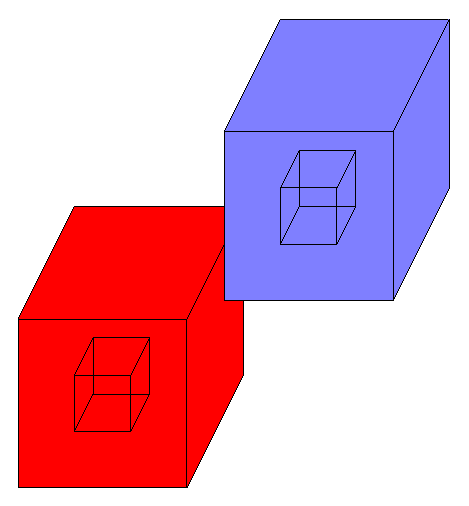
\includegraphics[width=1.2in]{images/config3D_3_2_2_3x3x3.eps} \\
(d) $\gDim{3}$ regions. & (e) $\gDim{3}$ regions.
  & (f) $\gDim{3}$ regions.\\
Configuration (3,2,0). & Configuration (3,2,1). 
  & Configuration (3,2,2).
\end{tabular}
\caption{Problematic 3D configurations of selected cubes.}
\label{fig:loose3D}
\end{figure*}

\begin{figure}[t]
\centering

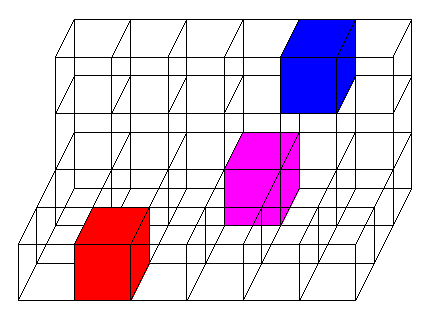
\includegraphics[width=1.2in]{images/config3D_3_2_2_B.eps}

\caption{Problematic interaction of red and blue cubes
in configuration (3,2,2) is blocked by magenta cube.}
\label{fig:blocked3D}
\end{figure}

Some examples of tightly packed 3D configurations of cubes are given
in Figure~\ref{fig:packed3D}.
Any line segment with endpoints in the two selected cubes $\cb$ and $\cb'$
will be well contained within the union 
of the two $3 \times 3 \times 3$ regions, 
$\RIII_\cb$ and $\RIII_{\cb'}$, around $\cb$ and $\cb'$.

Figure~\ref{fig:loose3D} contains three problematic configurations,
$(3,2,0)$, $(3,2,1)$ and $(3,2,2)$,
of  selected cubes.
Line segments with endpoints in the two selected cubes $\cb$ and $\cb'$
may contain points outside $\RIII_\cb \cup \RIII_{\cb'}$.
SHREC attempts to avoid selecting cubes with these configurations.

If two selected cubes, $\cb$ and $\cb'$, 
are in configuration $(2,2,0)$, $(2,2,1)$ or $(2,2,2)$,
then a line segment with endpoints in $\cb$ and $\cb'$
could intersect the boundary of $\RIII_\cb \cup \RIII_{\cb'}$.
Such configurations are undesirable.
Unfortunately, we found that avoiding such configurations is too restrictive.

Consider two cubes, $\cb$ and $\cb''$ 
in a $(3,2,0)$, $(3,2,1)$ or $(3,2,2)$ configuration.
If a third selected cube $\cb'$ lies between $\cb$ and $\cb''$,
then the 1-dimensional feature will pass from $\cb$ to $\cb'$ to $\cb''$.
The selection of $\cb'$ ``blocks'' the problematic interaction 
of $\cb$ and $\cb''$.
If cubes $\cb$ and $\cb'$ are selected,
then SHREC will permit the selection of $\cb''$,
even though $\cb$ and $\cb''$ have a configuration $(3,2,*)$.
Figure~\ref{fig:blocked3D} contains an example of two cubes 
in a $(3,2,2)$ configuration and a third cube between them.

More formally,
let $\cb$, $\cb'$ and $\cb''$ be grid cubes with grid indices
$(x_0,x_1,x_2)$, $(x'_0,x'_1,x'_2)$ and $(x''_0,x''_1,x''_2)$, respectively.
Cube $\cb'$ {\em separates} $\cb$ from $\cb''$
if $x'_i \in [x_i,x''_i]$ for $i = 0,1,2$
and $x_i < x'_i < x''_i$ or $x_i > x'_i > x''_i$ for some $i$.
SHREC avoids selecting cube $\cb''$ if some already selected cube $\cb$
forms a $(3,2,0)$ or $(3,2,1)$ or $(3,2,2)$ configuration with $\cb''$
and no already selected cube separates $\cb$ from $\cb''$.

\begin{figure}
\begin{equation*}
\xymatrix{
\action{Select 0D feature cubes} \ar[d] \\
\action{Select 1D features cubes in $7 \times 7 \times 7$ regions \\
around selected 0D feature cubes} \ar[d] \\
\action{Select 1D feature cubes whose indices are congruent \\
to $(0,0,0) \bmod 6$.} \ar[d] \\
\action{Select 1D feature cubes whose indices are congruent \\
to permutations of $(k,0,0) \bmod 6$.} \ar[d] \\
\action{Select 1D feature cubes whose indices are congruent \\
to permutations of $(k_a,k_b,0) \bmod 6$.} \ar[d] \\
\action{Select 1D feature cubes whose indices are congruent \\
to permutations of $(k_a,k_b,k_c) \bmod 6$.}
}
\end{equation*}
\caption{SHREC algorithm for selecting 0D and 1D feature cubes.}
\label{alg:SHREC_select}
\end{figure}

Figure~\ref{alg:SHREC_select} contains an outline of the algorithm 
for selecting 0D and 1D feature cubes.
SHREC first selects 0D feature cubes.
When the 0-dimensional feature is inside an active cube,
SHREC selects the active cube containing the feature point.
When the feature point is not in an active cube,
SHREC selects the active cube ``closest'' to the feature point
by choosing the cube $\cb$ whose center has minimum $L_\infty$ distance
to the feature point.

SHREC next selects 1D feature cubes which are ``near'' 
the selected 0D feature cubes,
i.e., they are contained in an $7 \times 7 \times 7$ region
around each selected 0D feature cube.
Selecting 1D feature cubes near 0D feature cubes poses special challenges
since there are multiple 1-dimensional features ending 
at a 0-dimensional feature.
Selecting a cube which is near two such 1-dimensional features.
can obscure one of the edges.

Let $\cb$ be a selected 0D feature cube and let $\cb'$ be a 1D feature cube
which is in a $(2,0,0)$, $(2,1,0)$ or $(2,1,1)$ configuration with $\cb$.
Let $\cb''$ be any cube sharing an edge or facet with $\cb'$
which is contained in the $5 \times 5 \times 5$ region
but is not covered by $\cb$.
If $\cb''$ is active and a 1D feature cube,
then SHREC attempts to avoid selecting cube $\cb'$.

Once 1D feature cubes near 0D feature cubes are selected,
SHREC could iterate by selecting uncovered 1D feature cubes 
near already selected cubes.
If no uncovered 1D feature cubes was near a selected cube,
SHREC could select an arbitrary uncovered 1D feature cube
and extend the set of selected cubes from that cube.
By not selecting a cube $\cb''$ 
if it forms a $(3,2,0)$, $(3,2,1)$ or $(3,2,2)$
with an already selected cube $\cb$ 
(and is not separated by a selected cube from $\cb$,)
SHREC would produce a tight packing of selected cubes.

\suppressfloats

\begin{figure}[t]
\centering

\begin{tabular}{cc}
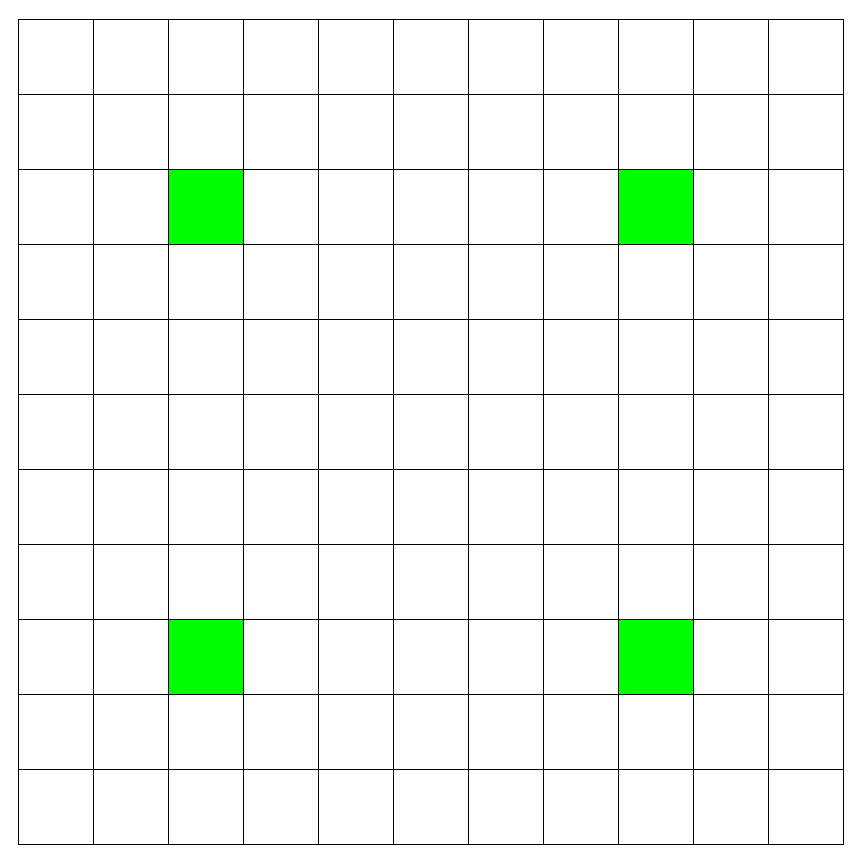
\includegraphics[width=0.4\linewidth]{images/mod6.eps} \qquad &
\qquad
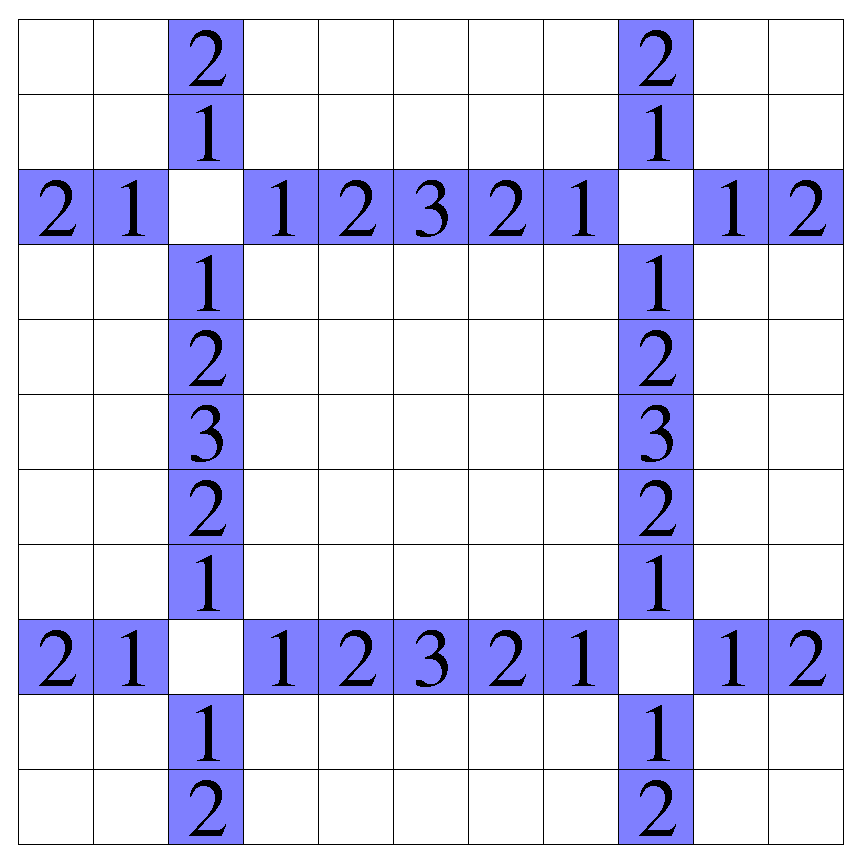
\includegraphics[width=0.4\linewidth]{images/mod6_k_0.eps} \\
(a) & (b)
\\
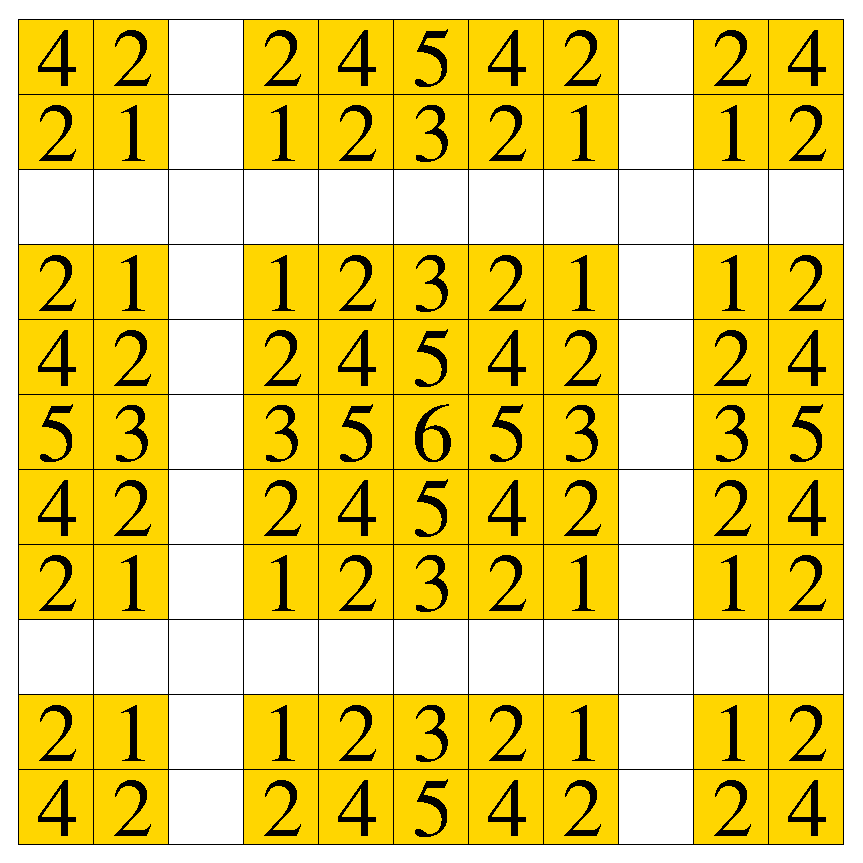
\includegraphics[width=0.4\linewidth]{images/mod6_ka_kb.eps} \qquad &
\\
(c)
\end{tabular}

\caption{2D illustration of order of cube selection based 
on cube indices mod 6.
(a) Green squares are $(0,0) \bmod 6$.
(b) Blue squares are $(k,0) \bmod 6$ or $(0,k) \bmod 6$ for $k=1,\ldots,5$.
Squares marked 1 are selected first, then squares marked 2
and then squares marked 3.
(c)~Yellow squares are $(k_a,k_b) \bmod 6$ for $k_a=1,\ldots,5$
and $k_b=1,\ldots,5$.
Squares marked 1 are selected first, then squares marked 2,
then 3, 4 and 5.
}
\label{fig:mod6}
\end{figure}

The algorithm outlined in the previous paragraph would produce
a good set of selected cubes but it is highly sequential.
One of the best aspects of the Marching Cubes and dual contouring algorithms
is their local, distributed, paralellizable nature.
Sequentially extending the set of selected cubes would totally destroy
that aspect of the algorithms.
Instead of selecting cubes using the sequential algorithm given above,
SHREC divides the regular grid 
into overlapping $6 \times 6 \times 6$ regions,
selects cubes from the boundaries of those regions and then from their interior.
The algorithm is completely local and easily distributed and parallelizable.

Each grid cube has an index $(x_0, x_1, x_2)$.
SHREC processes the grid cubes by reducing the indices modulo six
to $(x_0 \bmod 6, x_1 \bmod 6, x_2 \bmod 6)$ (Figure~\ref{fig:mod6}(a)).
SHREC first selects 1D feature cubes 
with indices congruent to $(0,0,0)$ modulo six.
SHREC next selects 1D feature cubes with indices congruent modulo six
to $(\pm 1,0,0)$ or $(0, \pm 1, 0)$ $(0, 0, \pm 1)$.
(Figure~\ref{fig:mod6}(b)).
SHREC then selects 1D feature cubes with indices congruent modulo six
to $(\pm 2,0,0)$ or $(0, \pm 2, 0)$ $(0, 0, \pm 2)$.
Finally, SHREC selects 1D feature cubes with indices congruent modulo six
to $(3,0,0)$ or $(0, 3, 0)$ $(0, 0, 3)$.
SHREC does not select a 1D feature cube $\cb$ 
if some already selected cube $\cb'$.
forms configuration $(3,2,0)$, $(3,2,1)$ or $(3,2,2)$ with $\cb$
and no already selected cube separates $\cb$ from $\cb''$.

SHREC next selects 1D feature cubes which are some permutation
of $(k_a,k_b,0)$ modulo six,
starting first with permutations of $(\pm 1, \pm 1, 0)$
and ending with permutations of $(3, 3, 0)$.
(Figure~\ref{fig:mod6}(c)).
Finally, SHREC selects 1D feature cubes which are permutations
$(k_a, k_b, k_c)$ modulo six,
starting first with permutations of $(\pm 1, \pm 1, \pm 1)$
and ending with $(3, 3, 3)$.

It is possible that the selection of two 1D feature cubes $\cb$ and $\cb''$
at distance five apart can force the selection of an edge cube $\cb'$
which has a $(3,2,1)$ or $(3,2,2)$ configuration 
with either $\cb$ or $\cb''$.
This happens if the distance vector between $\cb$ and $\cb''$
is $(5,3,2)$.
Thus, in addition to avoiding $(3,2,*)$ configurations,
SHREC also avoids selecting two cubes, $\cb$ and $\cb''$, 
which form a $(5,3,2)$ configuration.
Of course, if $\cb$ and $\cb''$ are separated by some other selected cube,
then they can both be selected.

While the above rules select a set of cubes which almost completely cover
the 1-dimensional features of a surface,
it is possible that the configuration restrictions leave a few areas uncovered.
Therefore, SHREC repeats the selection process to select any remaining
uncovered 1D feature cubes but drops the configuration restrictions.


\section{Merging Points with Features Points}
\label{section:merging}

Algorithm MergeSharp merges neighbors of a selected cube $\cb$ 
with $\cb$ when $\cb$ is selected.
This merging step sometimes created extremely thin triangles and 
sometimes flips triangle orientations.
SHREC is much more careful about its cube merging.
SHREC also extends the merging to some cubes in a $5 \times 5 \times 5$ region 
around each selected cube.
Note that SHREC actually merges the isosurface vertices generated by the cubes,
not the cubes themselves.

SHREC relies upon some angle tests to determine permissible merging.
Before performing such tests, SHREC maps the grid 
and the computed isosurface locations $\cb.\isovLoc$
to the regular grid composed of unit cubes.

\subsection{Ordered Merging}
\label{section:ordered_merging}

SHREC first merges neighbors of selected 0D feature cubes.
SHREC merges these neighbors in three steps.
First, for each selected 0D feature cube $\cb$,
SHREC merges with $\cb$ the active cubes which share a facet with $\cb$.
Next, for each selected 0D feature cube $\cb$,
SHREC merges with $\cb$ the active cubes which share an edge with $\cb$.
Finally, for each selected 0D feature cube $\cb$,
SHREC merges with $\cb$ the active cubes which share a vertex with $\cb$.
Of course, once an active cube is merged with some selected cube,
it is never merged with any other cube.

SHREC next merges neighbors of selected 0D feature cubes.
The procedure is similar to the one for 0D feature cubes.
SHREC first merges active cubes which share a facet with a selected 1D feature cube,
then merges active cubes which share an edge with a selected 1D feature cube,
and finally merges active cubes which share a vertex 
with a selected 1D feature cube.


\begin{figure}[t]
\centering

\begin{tabular}{cc}
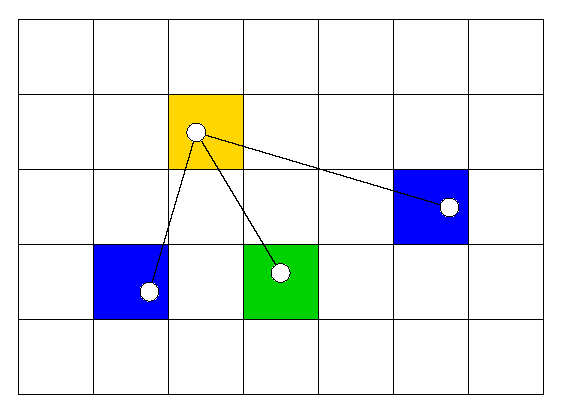
\includegraphics[width=1.2in]{images/connectedToIII.eps} \quad &
\quad
\includegraphics[width=1.2in]{images/manifold_problem_annotated.eps} \\
(a) & (b)
\end{tabular}

\caption{(a)~Isosurface in yellow square is connected to three selected cubes.
Yellow square should merge with the middle green square,
not with either of the blue squares.
(b)~Merging the red vertex with either of the yellow vertices
will cause the yellow edge to be contained in four polygons.}

\label{fig:connectedToIII}
\label{fig:manifold_problem}
\end{figure}

\subsection{Merging Tests}
\label{section:merging_tests}

For both the 0D feature cube and 1D feature cube merging,
SHREC applies six different tests to avoid creating very thin triangles
or flipping triangles or violating manifold conditions.
Consider a cube $\tcb$ which SHREC would like to merge 
with a selected cube $\cb$.
In order for a cube $\tcb$ to merge with a selected cube $\cb$,
cubes $\tcb$ and $\cb$ should satisfy the following conditions:
\begin{enumerate}
\item Some isosurface edge connects $\tcb$ to $\cb$.
\item Merging $\tcb$ with $\cb$ does not create an edge 
which is contained in four isosurface triangles or quadrilaterals
(manifold condition).
\item If $\tcb$ is connected to three different selected 1D feature cubes,
$\cb$, $\cb'$ and $\cb''$,
then $\cb$ should lie ``between'' $\cb'$ and $\cb''$.
(See Figure~\ref{fig:connectedToIII}(a) for a 2D illustration.)
\item Merging $\tcb$ with $\cb$ does not create a triangle
with very small angles.
\item Merging $\tcb$ with $\cb$ does not ``flip'' a triangle,
creating a ``fold'' in the isosurface.
\item If $\tcb$ has two or more isosurface vertices,
and an adjacent cube $\tcb'$ has one isosurface vertex
and shares an ambiguous facet with $\tcb$,
then $\tcb'$ should merge with $\cb$.
\end{enumerate}
We describe these conditions in more detail below.

First, SHREC checks that the isosurface vertex in $\tcb$
is connected to the isosurface vertex in $\cb$.
A cube $\tcb$ is connected to a selected cube $\cb$
if $\tcb$ shares an active facet or edge with $\cb$
or some cube $\tcb'$ shares an active facet or edge with $\tcb$ and
is merged with $\cb$.
If $\tcb$ is not connected with $\cb$, then $\tcb$ is not merged with $\cb$.

Second, SHREC checks for some manifold violations that
could be caused by merging $\tcb$ with $\cb$.
For each such selected cube $\cb' \neq \cb$ which is connected to $\tcb$,
SHREC checks if $\cb'$ is connected to $\cb$.
Let $\cb'$ be a selected cube which is connected to $\cb$ and $\tcb$.
Each active edge $\eb$ of $\tcb$ is dual to an isosurface quadrilateral
with a vertex in $\tcb$.
Let $\tcb_1$, $\tcb_2$, and $\tcb_3$ be the three other cubes containing $\eb$.
If some $\tcb_i$ merges with $\cb$ and another $\tcb_j$ merges with $\cb'$,
then merging $\tcb$ with $\cb$ collapses this quadrilateral to a triangle
or an edge.
However, if no isosurface quadrilateral dual to an active edge of $\tcb$
has vertices in $\tcb$, $\cb$ and $\cb'$,
then merging $\tcb$ with $\cb$ creates a non-manifold edge 
from $\cb$ to $\cb'$ with four incident polygons.
(See Figure~\ref{fig:manifold_problem}(b).)
If some selected $\cb'$ is connected to both $\cb$ and $\tcb$,
but no isosurface quadrilateral has vertices in $\tcb$, $\cb$ and $\cb'$,
then SHREC does not merge $\tcb$ with $\cb$.

Third, SHREC checks that if $\tcb$ is connected to three selected 1D feature cubes,
$\cb$, $\cb'$ and $\cb''$, then $\cb$ is between $\cb'$ and $\cb''$.
If not, then mapping $\tcb$ to $\cb$ could create a triangle 
with a small angle.
(See Figure~\ref{fig:connectedToIII} for a 2D illustration.)
Let $\cb$, $\cb'$ and $\cb''$ be grid cubes with grid indices
$(x_0,x_1,x_2)$, $(x'_0,x'_1,x'_2)$ and $(x''_0,x''_1,x''_2)$, respectively.
If $(x''_0,x''_1,x''_2)$ is contained in the box with corners
$(x_0,x_1,x_2)$ and $(x'_0,x'_1,x'_2)$ and does not lie on any 
of the eight corners of that box,
then we say that $\cb''$ lies between $\cb$ and $\cb'$.
If $\tcb$ is connected to selected 1D feature cubes $\cb$, $\cb'$ and $\cb''$,
and $\cb''$ lies between $\cb$ and $\cb'$
or $\cb'$ lies between $\cb$ and $\cb''$
then SHREC does not merge $\tcb$ with $\cb$.

In the fourth and fifth tests,
SHREC checks whether mapping $\tcb$ to $\cb$ creates an isosurface triangle 
with a small angle or ``flips'' an isosurface triangle,
creating a ``fold'' in the isosurface.
These tests are a little more complicated than the others
and are explained in the next section.

Finally, SHREC checks whether cube $\tcb$ has more than one isosurface vertex.
If cube $\tcb$ has more than one isosurface vertex,
then it has at least one ambiguous facet.
(A facet is ambiguous if two diagonally opposite vertices have
scalar value above the isovalue while the other two vertices
have scalar value below the isovalue.)
Let $\tcb'$ be a cube sharing an ambiguous facet with $\tcb$.
If cube $\tcb$ has only one isosurface vertex and 
$\tcb'$ is not merged with $\cb$, then $\tcb$ is not merged with $\cb$.

\subsection{Distortion Tests}
\label{section:distortion_tests}

Let $q$ be a quadrilateral dual to some active edge of $\tcb$.
Let $\tw$ be the vertex of $q$ which is generated by $\tcb$.
Quadrilateral $q$ can either be triangulated by adding a diagonal
incident on $\tw$ or by adding a diagonal connecting the neighbors
of $\tw$ in $q$.
Triangulating $\tw$ by adding a diagonal incident on $\tw$
places more restrictions on possible locations of $\tw$.
Since SHREC does not know how $q$ will be triangulated,
it assumes this more restrictive triangulation.

The diagonal of $q$ incident on $\tw$ splits $q$ into two triangles.
SHREC checks whether mapping $\tcb$ to $\cb$ will severely distort
either of those triangles.
Let $\tcb$, $\tcb'$ and $\tcb''$ be the cubes 
containing the triangle vertices.
SHREC only checks triangles where $\tcb'$ and $\tcb''$ 
are not covered or selected.

Let $\tw$, $\tw'$ and $\tw''$ be the vertices generated
by $\tcb$, $\tcb'$ and $\tcb''$.
Let $w$ be the vertex generated by selected cube $\cb$.
In the fourth test,
SHREC computes $\angle(w,\tw',\tw'')$ and $\angle(w,\tw'',\tw')$.
If $\angle(w,\tw',\tw'')$ or $\angle(w,\tw'',\tw')$ is less than $5^\circ$,
then SHREC does not map $\tcb$ to $\cb$.

The fifth test is composed of two different parts.
In the first part,
SHREC checks whether mapping $\tw$ to $w$
significantly changes the normal of triangle $(\tw,\tw',\tw'')$.
If the angle between the normal of $(w, \tw', \tw'')$ is less than $30^\circ$,
then the triangle passes this test.

In the second part, SHREC checks the orientation of $(w, \tw', \tw'')$.
Let $\eb$ be the grid edge shared by cubes $\tcb$, $\tcb'$ and $\tcb''$.
Let $\pi(w)$, $\pi(\tw')$ and $\pi(\tw'')$ be the orthogonal projection
of $w$, $\tw'$ and $\tw''$, respectively, 
onto a plane $h$ perpendicular to $\eb$.
If the orientation of $\pi(w)$, $\pi(\tw')$ and $\pi(\tw'')$
matches the orientation of $\tcb$, $\tcb'$ and $\tcb''$ around $\eb$,
then triangle $(w,\tw',\tw'')$ passes the orientation test.

To pass the fifth test,
SHREC requires that a triangle pass either the normal or the orientation test,
not necessarily both tests.
The original triangle $(\tw,\tw',\tw'')$ could have a normal which
is very far from the true surface normal.
In that case, the normal of triangle $(w, \tw', \tw'')$ should
be far from the normal of triangle $(\tw, \tw', \tw'')$.
On the other hand,
the projected vertices $\pi(w)$, $\pi(\tw')$ and $\pi(\tw'')$
could be nearly collinear.
In that case, $\pi(w)$, $\pi(\tw')$ and $\pi(\tw'')$ could have
opposite orientation from $\tcb$, $\tcb'$ and $\tcb''$,
even though the normal of $(w,\tw',\tw'')$ is quite close
to the original.


\subsection{Pair Merging}
\label{section:pair_merging}

A cube $\tcb$ may fail to merge with a selected cube $\cb$
because of some neighboring cube $\tcb'$
while $\tcb'$ fails to merge with $\cb$ because of $\tcb$.
Often this ``deadlocking'' arises when $\tcb$ and $\tcb'$ share
a common ambiguous facet.

After attempting to merge individual cubes,
SHREC tries to merge pairs $(\tcb,\tcb')$ of covered cubes with selected cubes.
The elements of the pairs should share a common facet or edge
and should both be covered by the selected cube $\cb$.
SHREC temporarily merges $\tcb$ with $\cb$,
and then applies all the above tests to $\tcb'$.
SHREC then temporarily merges $\tcb'$ with $\cb$,
and applies all the above tests to $\tcb$.
If both $\tcb$ and $\tcb'$ pass the tests,
then SHREC merges both of them with $\cb$.

As the merging proceeds,
it is possible that a cube which was previously unable 
to merge with any selected cube
is now able to merge with some such cube.
Thus, SHREC reapplies the algorithm in Section~\ref{section:ordered_merging}
and in this section to any remaining covered, unmerged cubes.


\subsection{Extended Merging}
\label{section:extended_merging}

The merging of cubes in $3 \times 3 \times 3$ region
around each selected cube will clear most but not all of the vertices 
around sharp features.
There are multiple reasons that some vertices 
near sharp features may remain.
First, the location of some vertex outside of $\RIII_\cb$
may stop some cube covered by $\cb$ from merging with $\cb$.
Second, if two selected $\cb$ and $\cb'$ are 
in a $(2,2,0)$ or $(2,2,1)$ or $(2,2,2)$ configuration, 
then a 1-dimensional feature with endpoints in $\cb$ and $\cb'$ can intersect
the boundary of the $\RIII_\cb \cup \RIII_{\cb'}$.
Vertices in uncovered can be arbitrarily close to such a 1-dimensional feature.
Third, while the selection step avoids most $(3,2,*)$ configurations,
it does not avoid all of them.
If $\cb$ and $\cb'$ are in a $(3,2,*)$ configurations,
then a 1-dimensional feature passing through $\cb$ and $\cb'$ 
may contain points outside of $\RIII_\cb \cup \RIII_{\cb'}$.

To handle such problems, SHREC extends the merging to cubes
in a $5 \times 5 \times 5$ region around each selected cube.
Merging cubes in a $5 \times 5 \times 5$ region $\RV_\cb$
around a selected cube $\cb$ can create its own problems 
of thin or flipped triangles.
Thus, SHREC only attempts to merge cubes in $\RV_\cb$
which are potentially near a 1-dimensional feature through $\cb$.

First, SHREC checks whether any covered cubes are unmerged
after the steps in Sections~\ref{section:ordered_merging}
and~\ref{section:pair_merging}.
If some cube $\tcb$ is covered by selected cube $\cb$
but not merged with any cube,
SHREC pairs $\tcb$ with any adjacent active cubes $\tcb'$
sharing a vertex with $\tcb$
and attempts to merge the pair $(\tcb,\tcb')$ with $\cb$.
SHREC applies the pair merging procedure
in Section~\ref{section:pair_merging} to determine whether
to allow the pair $(\tcb,\tcb')$ to merge with $\cb$.
Note that in Section~\ref{section:pair_merging} both cubes in the pair
must be contained in $\RIII_\cb$ while here only one cube
must be contained in $\RIII_\cb$.

It is possible that the interaction of vertices in three cubes
prevents a covered cube from merging with a selected cube.
SHREC considers triples of unmerged cubes
which share a common edge $\eb$.
At least one cube in the triple must be in $\RIII_\cb$.
The triple merging procedure is similar to the pair merging procedure
described in Section~\ref{section:pair_merging} and is omitted.

Next, SHREC tries to merge cubes which lie 
at the intersection $\partial \RIII_\cb \cap \RIII_{\cb'}$
of two $\gDim{3}$ regions around two selected cubes $\cb$ and $\cb'$.
More specifically, SHREC attempts to merge a cube $\tcb$ 
with a selected cube $\cb$ if some facet of $\tcb$ lies 
on the boundary of $\RIII_\cb$ 
while some other facet of $\tcb$ lies on the boundary of $\RIII_{\cb'}$.
Note that such a cube is contained in $\RV_\cb$.
SHREC applies all the tests in Section~\ref{section:merging_tests}
to determine whether to merge $\tcb$ with $\cb'$.

Finally, SHREC tries to merge pairs of cubes $(\tcb, \tcb')$ which lie
at the intersection $\partial \RIII_\cb \cap \RIII_{\cb'}$.
Both $\tcb$ and $\tcb'$ must have facets which lie on $\RIII_\cb$
and $\RIII_{\cb'}$.
SHREC applies the pair merging procedure described 
in Section~\ref{section:pair_merging} to determine whether
to allow the pair $(\tcb,\tcb')$ to merge with $\cb$.


\begin{figure}[t]
\centering

\begin{tabular}{cc}
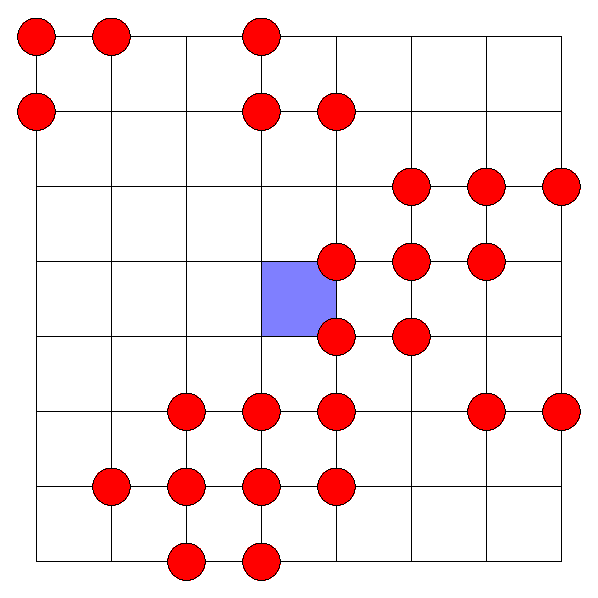
\includegraphics[width=0.4\linewidth]{images/undefined_grad_7x7x7.eps} \qquad &
\qquad
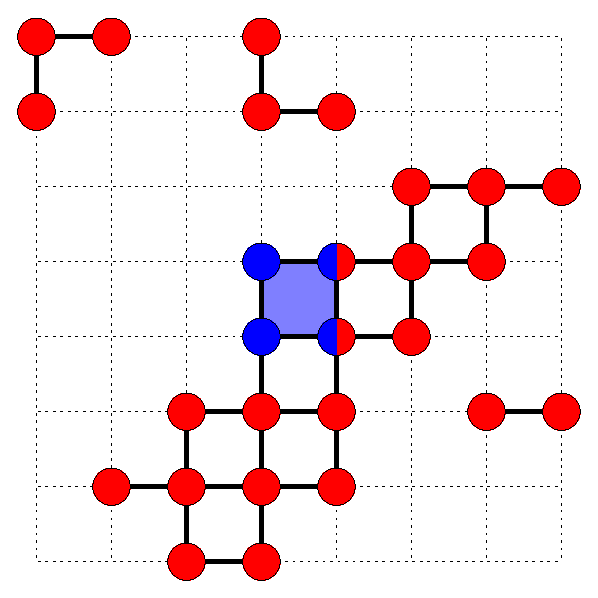
\includegraphics[width=0.4\linewidth]{images/ugrad_graph_7x7x7.eps} \\
(a) & (b) \\
\\
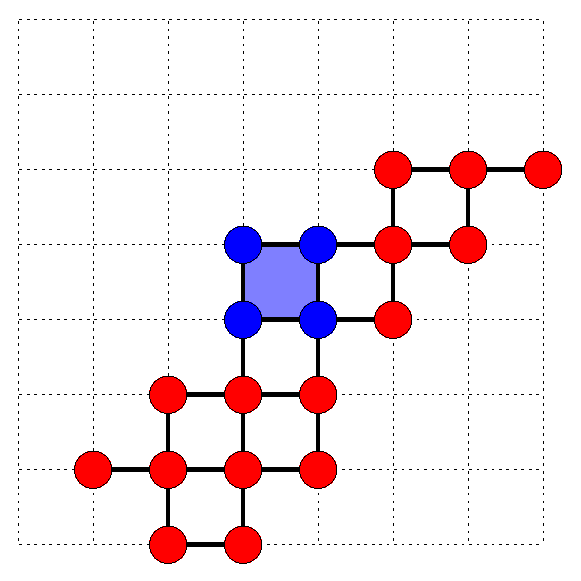
\includegraphics[width=0.4\linewidth]{images/ugrad_component_7x7x7.eps} \qquad &
\qquad
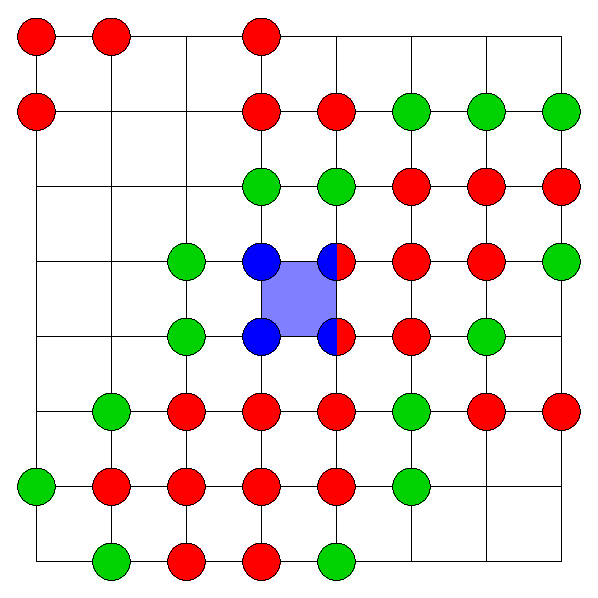
\includegraphics[width=0.4\linewidth]{images/selected_grad_7x7x7.eps} \\
(c) & (d) \\
\end{tabular}

\caption{2D example of selecting gradients ``close'' to square $\cb$.
(a)~Set $Q$ of red vertices with undefined gradients.
(b)~Graph $G_\cb$ formed from $Q \cup Q_\cb$ and the grid edges.
$Q_\cb$ is the set of four blue vertices of square~$\cb$.
(c) Connnected component $G'$ of $G_\cb$.
(d) Green vertices which are connected to the vertices of $G'$.
The green vertices are the vertices with defined gradients
which are ``close'' to $\cb$.
}
\label{fig:grad_select}
\end{figure}

\section{Selecting Gradients}
\label{section:gradients}

The algorithm in Section~\ref{section:loc}
for computing isosurface vertex locations requires
a set of gradients for each cube $\cb$.
An obvious set is the gradients at the vertices of $\cb$.
However, even if correct gradients were provided at every vertex of $\cb$,
this set would not suffice.
It is possible to have an active cube $\cb$
which contains a sharp isosurface corner
defined by three perpendicular planes
while only two of the planes are represented by the gradients of $\cb$.

MergeSharp computes isosurface vertex locations 
from the vertices of $\cb$ and of the six cubes sharing a facet with $\cb$.
When exact gradients are provided at all grid vertices,
this set of gradients suffices.

When gradients are not provided in the input,
they must be computed from the scalar data.
If an isosurface has sharp features,
then the gradient field is discontinuous around those sharp features.
As discussed in~\cite{bw-isifsd-15}, 
computing correct gradients near gradient field discontinuities
is extremely difficult.
In~\cite{bw-isifsd-15},
Bhattaca and Wenger give an algorithm for computing correct gradients
in the presence of gradient discontinuities, but the algorithm does
not compute correct gradients at all the grid vertices.
Instead, the algorithm returns a set of correct gradients
at some of the grid vertices while returning no gradient information
at other vertices.
Under suitable conditions,
the algorithm returns the correct gradient at any vertex
which is at least three edge lengths from any gradient discontinuity.

Because the algorithm in~\cite{bw-isifsd-15} 
does not return gradients near gradient discontinuities,
no gradient information may be available for the vertices 
of cubes which contain those discontinuities
or for neighbors of such cubes.
Thus, we must use gradients from a $\gDim{7}$ region around each cube $\cb$.

When scalar data is provided by computer tomography (CT),
then the scalar values near gradient discontinuities
may also be incorrect.
As discussed in~\cite{bw-isifsd-15},
we must go out even further to a $\gDim{9}$ region 
around each cube $\cb$ to get gradient information.

Only gradients which determine isosurface tangent planes near $\cb$
should be used in $\cb.\isovLoc$.
We use three tests on the vertices in a $\gDim{7}$ or $\gDim{9}$
region around $\cb$ to determine such gradients.
First, we are only interested in vertices which are near the isosurface.
Thus, we only choose vertices from edges
where one endpoint has scalar value below
the isovalue and one endpoint has scalar value at or above the isovalue.
Second, we are only interested in vertices whose gradients generate planes
which are close to $\cb$.
We construct a cube $\cb'$ of size $1.5 \times 1.5 \times 1.5$ centered at $\cb$
and only choose a vertex $v$ 
if the plane $h_v$ given by Equation~\ref{eqn:isoplane}
intersects $\cb'$.

Third, if vertices ``close'' to $\cb$ have been chosen,
then there is no reason to select vertices ``far'' from $\cb$.
In fact, choosing gradients at vertices ``far'' from $\cb$
in smooth, curved surfaces can cause the creation 
of non-existent sharp features in the isosurface.

To choose only vertices close to $\cb$,
we consider the set $Q$ of vertices 
of the $9 \times 9 \times 9$ (or $7 \times 7 \times 7$) subgrid,
whose gradients are undefined.
(See Figure~\ref{fig:grad_select}.)
We choose only vertices with defined gradients
which are adjacent to vertices in $Q$.

More precisely, let $Q$ be the set of vertices of the subgrid
whose gradients are undefined (Figure~\ref{fig:grad_select}(a)).
Let $Q_\cb$ be the vertices of $\cb$.
Let $G_\cb$ be the graph whose vertices are $Q \cup Q_\cb$
and whose edges are $(u,v)$ where $(u,v)$ is a grid edge
(Figure~\ref{fig:grad_select}(b)).
We find the connected component $G'$ of $G_\cb$ containing $Q_\cb$
(Figure~\ref{fig:grad_select}(c)).
A grid vertex $u \not\in V(G')$ is on the boundary of $G'$
if $(u,v)$ is a grid edge and $v$ is in $V(G')$.
As out third test, we only a choose a vertex if it is in $Q_\cb$
or if it is on the boundary of $G'$.
(Figure~\ref{fig:grad_select}(d)).

Applying the three tests gives a set of vertices and their gradients
which define planes.
We use those vertices and their gradients to compute $p_\cb$
as described in Section~\ref{section:loc}.


\section{Parameters}
\label{section:parameters}

Algorithm SHREC has two major parameters,
one determining the number of large singular values in matrix $A$
and the second determining the size of the $\gDim{k}$ region 
from which gradients are selected around each cube
(Section~\ref{section:gradients}).
The first parameter is a value $\epsilon$ between 0 and 1.
As noted in Section~\ref{section:loc},
a singular value $\sigma_i$ of matrix $A$ 
is large if $\sigma_i/\sigma_1$ is greater than or equal to $\epsilon$.
The number of large singular values determines whether a vertex
is on a sharp feature or a smooth region of the isosurface.
To the best of our knowledge, all algorithms which reconstruct surfaces 
with sharp features require some parameter
to distinguish the sharp features from the smooth regions of the surface.

The second parameter is an odd integer $k \ge 3$.
Each cube $\cb$ uses gradients from a $\gDim{k}$ around the cube
in selecting gradients for computing $\cb.\isovLoc$.
The size of $k$ depends upon the input data.
If correct gradients are provided at each grid vertex,
then $k$ should equal 3 for a $\gDim{3}$ region around each cube.
If gradients are computed from correct scalar values 
using the algorithm in~\cite{bw-isifsd-15},
then $k$ should equal 7 for a $\gDim{7}$ region around each cube.
If gradients are computed from CT data 
using the algorithm in~\cite{bw-isifsd-15},
then $k$ should equal 9 for a $\gDim{9}$ region around each cube.

SHREC uses three other constants:
one for the triangle test in selecting vertices,
one for the angle test in merging cubes
and a second for the normal test in merging cubes.
In the triangle test,
if selecting cube $\cb$ would possibly create a triangle between three
selected cubes with angle greater than $140^\circ$, 
cube $\cb$ is not selected.
In the angle test,
if merging cube $\tcb$ with $\cb$ would create a triangle with angle
less than $5^\circ$, then cube $\tcb$ is not selected.
In the normal test,
if merging $\tcb$ with $\cb$ would change the normal 
of some triangle $(\tw,\tw',\tw'')$ by less than $30^\circ$,
then merging $\tcb$ with $\cb$ does not distort triangle $(\tw,\tw',\tw'')$.

Because SHREC is based on the regular grid,
the constants used in all three of these tests do not depend 
upon the input data and should work well for any scalar fields.
Note that SHREC maps the input grid 
and the computed isosurface locations $\cb.\isovLoc$
to the regular grid composed of unit cubes
before applying any of the above tests.
